% !TEX root = ../main.tex
%% Copyright 2025 Oxford University Press
%%
%% This file is part of the 'oup-authoring-template Bundle'.
%% ---------------------------------------------
%%
%% It may be distributed under the conditions of the LaTeX Project Public
%% License, either version 1.3 of this license or (at your option) any
%% later version.  The latest version of this license is in
%%    https://www.latex-project.org/lppl.txt
%% and version 1.2 or later is part of all distributions of LaTeX
%% version 1999/12/01 or later.
%%
%% The list of all files belonging to the 'oup-authoring-template Bundle' is
%% given in the file `manifest.txt'.
%%
%% Template article for Oxford University Press's document class `oup-authoring-template'
%% with bibliographic references
%%

%%%CONTEMPORARY%%%
\documentclass[unnumsec,webpdf,contemporary,large]{oup-authoring-template}%
%\documentclass[unnumsec,webpdf,contemporary,large,numbered]{oup-authoring-template}% uncomment this line to get the numbered reference output
%\documentclass[unnumsec,webpdf,contemporary,medium]{oup-authoring-template}
%\documentclass[unnumsec,webpdf,contemporary,mediumone]{oup-authoring-template}
%\documentclass[unnumsec,webpdf,contemporary,small]{oup-authoring-template}

%%%MODERN%%%
%\documentclass[unnumsec,webpdf,modern,large]{oup-authoring-template}
%\documentclass[unnumsec,webpdf,modern,large,numbered]{oup-authoring-template}%   uncomment this line to get the numbered reference output
%\documentclass[unnumsec,webpdf,modern,medium]{oup-authoring-template}
%\documentclass[unnumsec,webpdf,modern,mediumone]{oup-authoring-template}
%\documentclass[unnumsec,webpdf,modern,small]{oup-authoring-template}

%%%TRADITIONAL%%%
%\documentclass[unnumsec,webpdf,traditional,large]{oup-authoring-template}
%\documentclass[unnumsec,webpdf,traditional,large,numbered]{oup-authoring-template}%   uncomment this line to get the numbered reference output
%\documentclass[unnumsec,webpdf,traditional,medium]{oup-authoring-template}
%\documentclass[unnumsec,webpdf,traditional,mediumone]{oup-authoring-template}
%\documentclass[namedate,webpdf,traditional,small]{oup-authoring-template}

%\onecolumn % for one column layouts

%\usepackage{showframe}

\graphicspath{{Fig/}}

% line numbers
%\usepackage[mathlines, switch]{lineno}
%\usepackage[right]{lineno}

\theoremstyle{thmstyleone}%
\newtheorem{theorem}{Theorem}%  meant for continuous numbers
%%\newtheorem{theorem}{Theorem}[section]% meant for sectionwise numbers
%% optional argument [theorem] produces theorem numbering sequence instead of independent numbers for Proposition
\newtheorem{proposition}[theorem]{Proposition}%
%%\newtheorem{proposition}{Proposition}% to get separate numbers for theorem and proposition etc.
\theoremstyle{thmstyletwo}%
\newtheorem{example}{Example}%
\newtheorem{remark}{Remark}%
\theoremstyle{thmstylethree}%
\newtheorem{definition}{Definition}

%\usepackage{draftwatermark}
%\SetWatermarkText{Draft}
%%Uncomment  \usepackage{draftwatermark} and \SetWatermarkText{Draft} to watermark your PDF as a draft
\begin{document}

\journaltitle{Bioinformatics}
\DOI{To be assigned}
\copyrightyear{2026}
\pubyear{20xx}
\vol{XX}
\issue{x}
\access{To be assigned}
\appnotes{Paper}

\firstpage{1}

%\subtitle{Subject Section}

\title[Short Article Title]{MMCDS: A Multi-Stage and Multi-Model Hybrid Screening Solution for Male Contraception}


\abstract{
The development of male contraceptives is a critical global priority in reproductive health, essential for advancing reproductive health systems and optimizing family planning decisions. However, current research on its molecular targets is limited by target complexity and the low efficiency of compound screening, which hampers clinical translation. This study proposes a multi-stage, multi-model hybrid screening solution (MMCDS) for male contraception. MMCDS first employs two attention-based affinity classification models for large-scale compound filtering. Subsequently, a contrastive learning-based affinity regression model is integrated to quantitatively evaluate the screened compounds. Systematic protein-binding assays and cellular functional tests were conducted on the top-ranked compounds. 4 lead molecules with strong clinical translational potential were successfully identified, with the best equilibrium dissociation constant reaching 10$^{-7}$M. Additionally, compared to existing state-of-the-art deep learning methods, the results indicate that our solution achieves a 3.80-10.23\% improvement in simulated screening performance.
} 

\keywords{male contraception, drug-target prediction, MEIOB, SPATA22, drug discovery}

% \keywords[Abbreviations]{abbreviation1, abbreviation2, abbreviation3, abbreviation4}

% \otherabstract[Additional Abstract]{Use this element for elements such as Graphical abstract, Lay summary, Translated abstract etc. Que cum aut etum qui ium dolupta ssequia autati odis demporepe ad et es alit rem repudaerae min et volorum re volupta nobit volectur aut fuga.}

% \otherabstract[Graphical Abstract]{\colorbox{black!20}{\hbox to 0.97\textwidth{\vbox to 50pt{}}}}

% \boxedtext{Key Messages}{
% \begin{itemize}
% \item Key boxed text here.
% \item Key boxed text here.
% \item Key boxed text here.
% \end{itemize}}

\maketitle

%\begin{epigraph}
%Epigraph text. Ximporem qui reperov idempedit modio. Bisto imagnatem quae aceptis
%nobitae quid eum rae adignis quias-sit vellacc uptatur sunt quis rentis eaquasit alia deliquam
%rec-to consed unt. Empor sum ratur ressimusdae. Nam fugiae.
%\source{Epigraph source}
%\end{epigraph}



% UNCOMMENT THE BELOW TWO LINES IN CASE YOU NEED NUMBERED FORMAT.
% \bibliographystyle{oup-plain}
% \bibliography{reference}




\begin{figure*}[ht!]
    \centering
    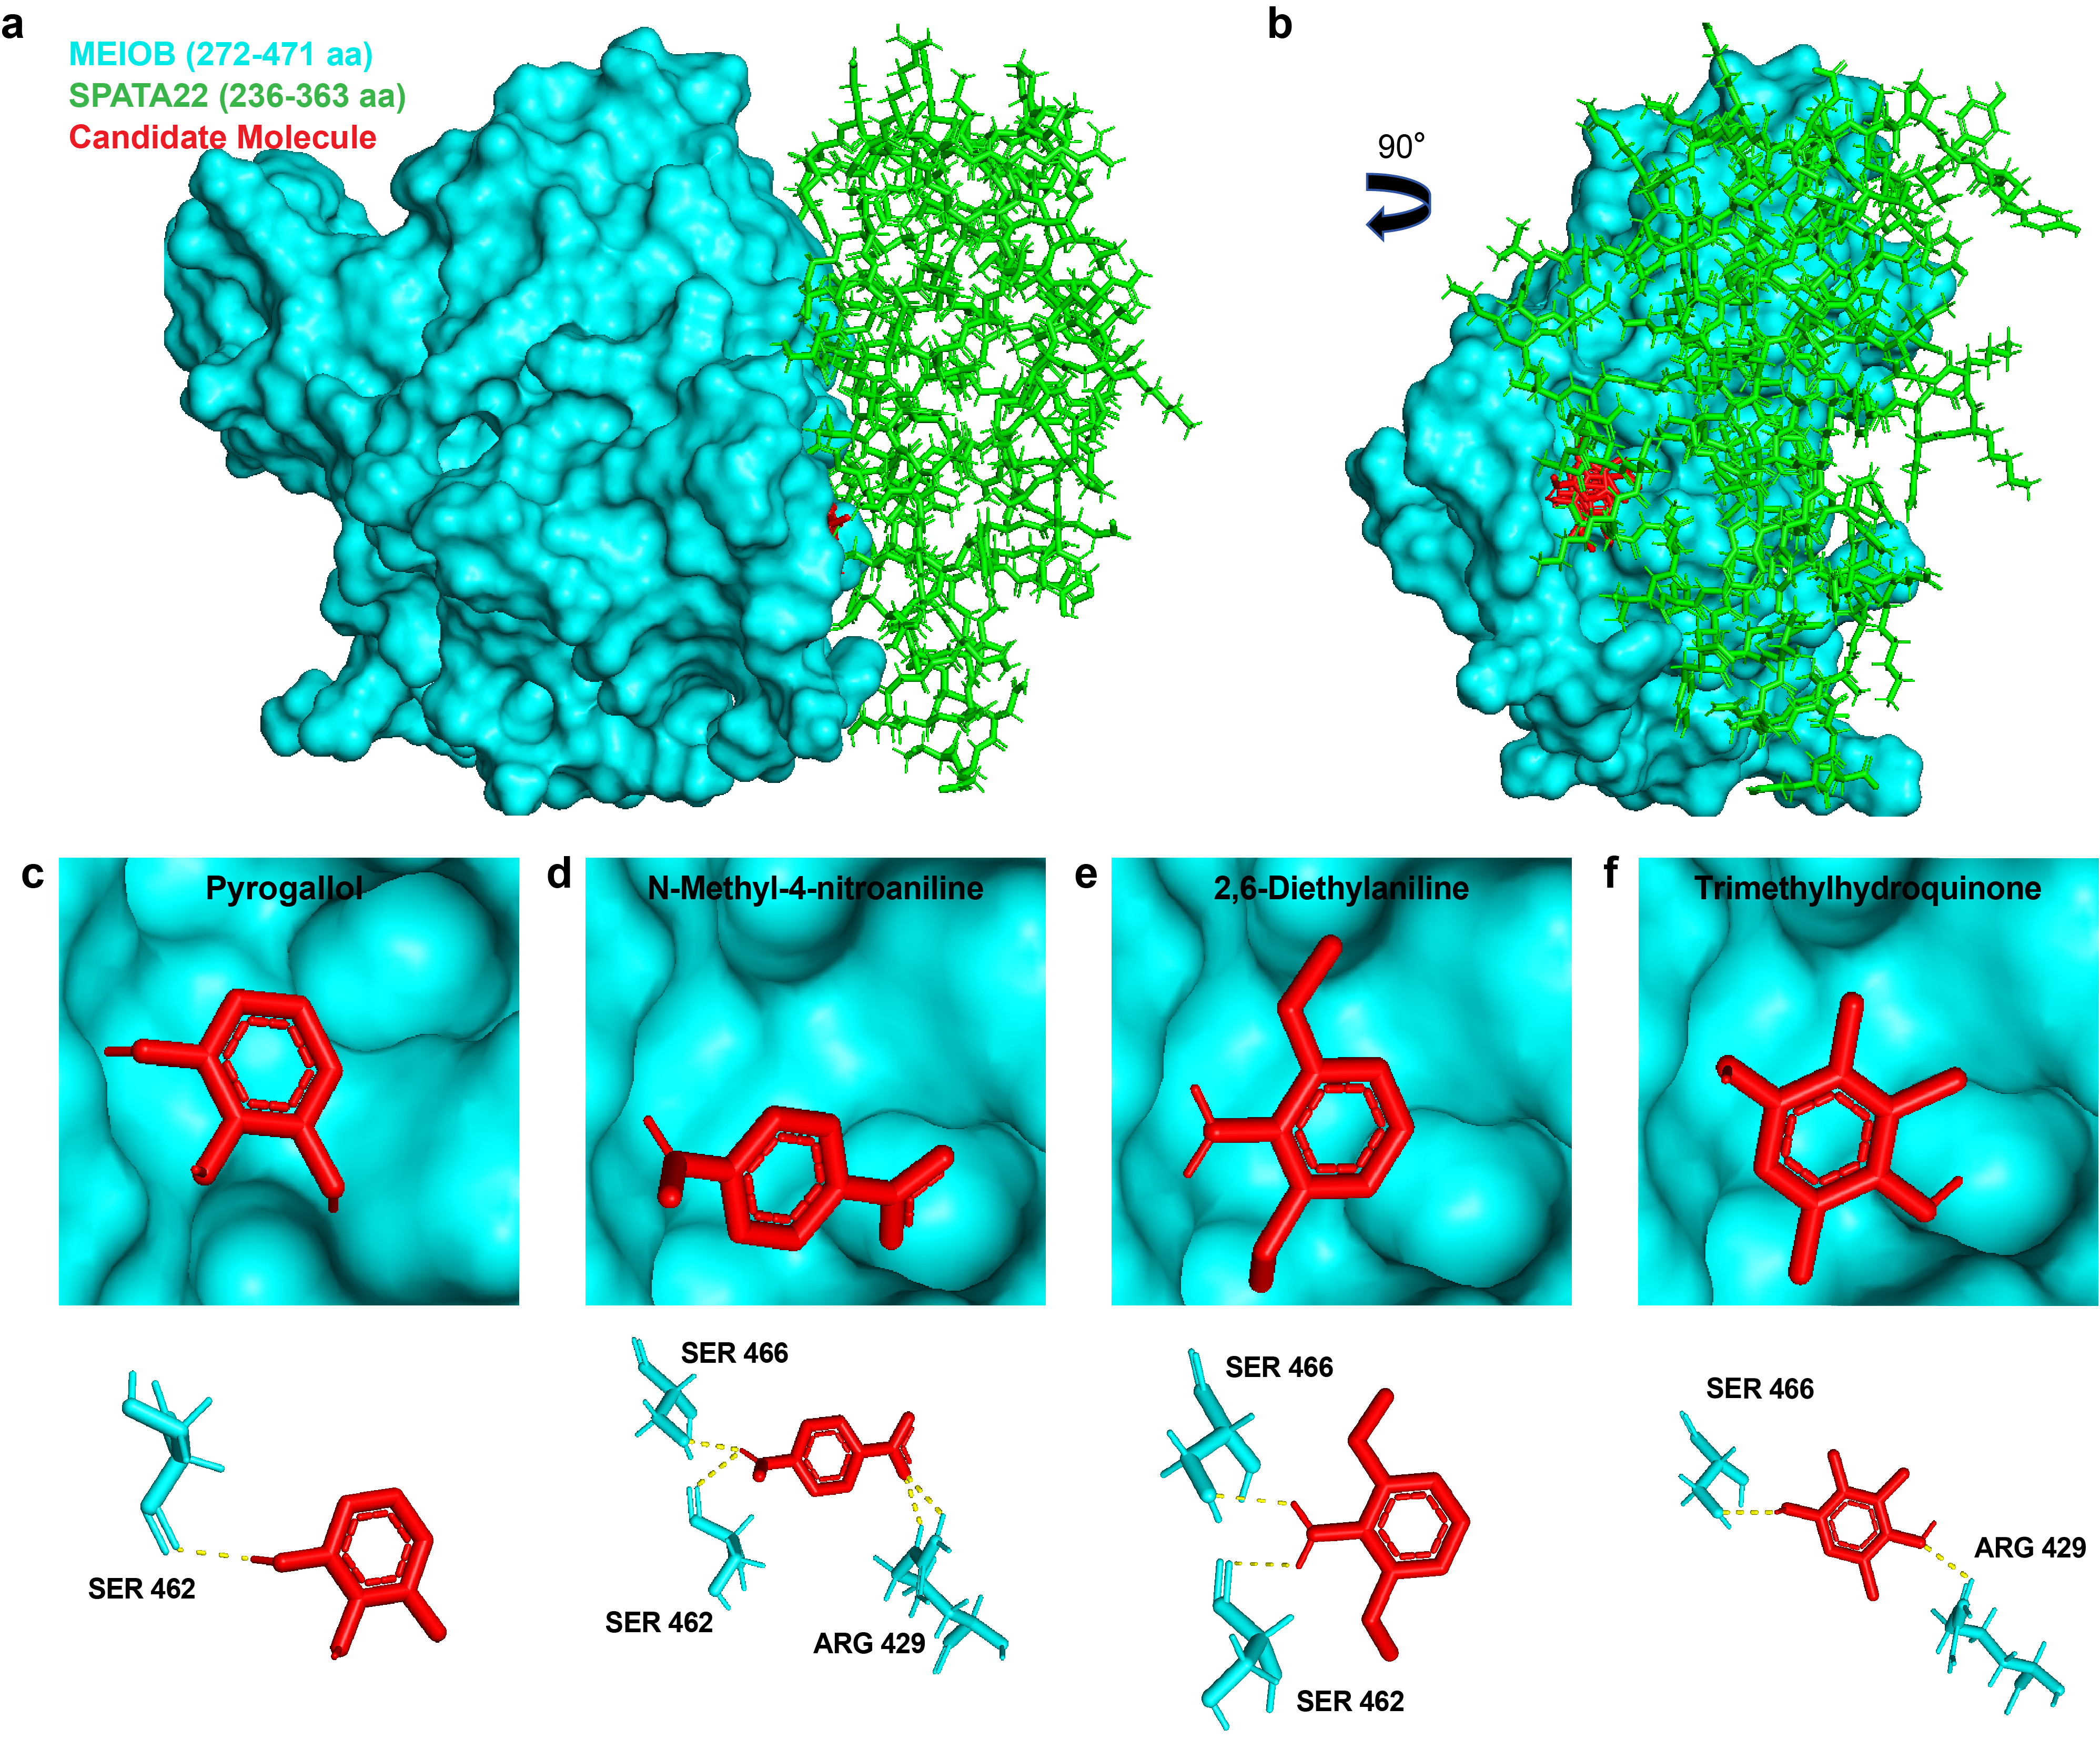
\includegraphics[width=1\linewidth]{pic/Fig S1.png}
    \caption{\textbf{Molecular docking simulation of small molecule with MEIOB (aa272-471) and SPATA22(aa236-363)}.
    \textbf{a-b} Preferential binding mode between compounds and MEIOB according to docking simulation using Pymol software.  \textbf{c} Preferential binding mode between Pyrogallol and MEIOB. \textbf{d} Preferential binding mode between N-Methyl-4-nitroaniline and MEIOB. \textbf{e} Preferential binding mode between 2,6-Diethylaniline and MEIOB. \textbf{f} Preferential binding mode between Trimethydroquinone and MEIOB. The amino acid residues involved in interactions are labeled. Cyan: MEIOB; Green: SPATA22; Red: Candidate molecules.}
    \label{fig:S1}
\end{figure*}



\section*{Appendix A: Methods}




\subsection*{Data collection}

Previously, we obtained a small molecule library capable of interacting with MEIOB-SPATA22 through high-throughput screening based on the intracellular bimolecular fluorescence complementation (BiFC) assay (\citealt{67}). Derived from Chembridge's Core set library, this compound library contains a total of 177 small molecules, which we classified as effective cases (Supplementary Table 1). Meanwhile, 42,956 samples in the ChemDiv and ChemBridge were viewed as ineffective cases during experiments. Additionally, on account of the fact that the effective cases have different binding abilities with MEIOB-SPATA22, we divided them into 19 true effective cases and 158 false counterparts with a threshold of $-4.2$ based on the distribution of effective cases.


\subsection*{Data Preprocessing}

In our experimental dataset, the number of confirmed positive samples (with specific reaction values) is substantially outnumbered by negative samples, resulting in a severe class imbalance that poses significant challenges for training effective classification or regression models directly. Therefore, during the screening stage for potentially effective molecules, we employ molecular fingerprint similarity to select the top k most similar negative samples for each positive sample. By maintaining a controlled positive-to-negative ratio during training, the model achieves more robust boundary discrimination.

Let the set of positive samples be $\text{D}_{\text{pos}}$ and the set of negative samples be $\text{D}_{\text{neg}}$. We define a similarity function $\text{SimFinger}(\cdot,\cdot)$ to compute the similarity between a positive sample $\text{D}_{\text{pos}}$ and a negative sample $\text{D}_{\text{neg}}$:
\begin{equation}
S(\text{D}_{\text{pos}}, \text{D}_{\text{neg}}) = \text{SimFinger}(F_{\text{pos}}, F_{\text{neg}})
\end{equation}
where $F_{\text{pos}}$ and $F_{\text{neg}}$ are the molecular fingerprint feature vectors of the positive and negative samples, respectively. The top $k$ negative samples are selected as follows:
\begin{equation}
N_k(p) = \{n \in N \,|\, S(p, n) \text{ is top } k \text{ for } p\}
\end{equation}

% 将177个有反应数值的数据整合到广泛使用的KIBA数据集中来增强数据集，并将所有测量值映射到合适的数值范围内。
During the data preprocessing for the ranking phase, there are 177 samples with regression numerical labels (\citealt{67}). Due to the limited sample size, we integrate these 177 response-valued data points into the widely used KIBA dataset to enhance the training data. All measured values are mapped to an appropriate numerical range through linear transformation.

Let $x_{\text{orig}} \in [a,b]$ represent the original values from our 177 samples, and $y \in [c,d]$ denote the KIBA score range. The linear mapping function is formulated as:
\begin{equation}
y = c + \left( \frac{x_{\text{orig}} - a}{b - a} \right) \times (d - c)
\end{equation}

This normalization ensures that the original measurements maintain their relative distribution while being aligned with the KIBA dataset's scale.


\subsection*{Cell culture}

HeLa, SiHa, MDA-MB-231, A2780, THP-1 and HEK 293T cells were purchased from American Type Culture Collection (ATCC). C33A cells were purchased from Wuhan Pusai Biotechnology Co., Ltd. Cells were cultured in DMEM (BasalMedia Technologies), MEM (Gibco) or RIPA-1640 (Gibco) supplemented with 10\% fetal bovine serum (FBS; AusGeneX) and 100 U/mL penicillin and streptomycin in a humidified 5\% CO$_2$ atmosphere. 


\subsection*{Protein expression and purification}
The full-length human MEIOB sequence was codon-optimized by using the Integrated DNA technologies\footnote{https://sg.idtdna.com/pages/} and synthesized by Sangon Biotech. The optimized full-length human MEIOB sequence was inserted into the \textit{Nde}I/\textit{Xho}I restriction sites of the pET-42b(+) vector (Addgene) with 8×His-Tag to construct the pET-42b-hMEIOB-8×His-Tag vector. DNA fragments encoding the CopGFP and mCherry tags were amplified from vectors pCDH-EF1-CopGFP (Addgene) and pCDH-EF1a-eFFly mCherry (Addgene), and then inserted into the \textit{Xho}I/\textit{Xba}I restriction sites of the pcDNA3.1(+) vector (Addgene) to generate pcDNA3.1-CopGFP-C and pcDNA3.1-mCherry-C. The optimized full-length human MEIOB and SPATA22 fragments were inserted into the \textit{Nhe}I/\textit{Xho}I sites of pcDNA3.1-CopGFP-C or pcDNA3.1-mCherry-C. The vectors were constructed and extracted with an EndoFree Mini Plasmid Kit II (TIANGEN). The purified plasmid was transfected into HEK 293T cells with LipofectamineTM 2000 Transfection Reagent (Thermo Fisher). After 8 h, candidate drugs prepared in low-serum medium were added, and the culture was continued for another 48 h. Subsequently, the samples were mounted with mounting medium containing DAPI, followed by observation and photography under the fluorescence microscope (ApoTome.2; ZEISS).

\subsection*{Protein expression and purification}

The plasmids pET-42b-hMEIOB-8×His-Tag were transformed into the bacterial strain E. coli BL21 for protein production. A single colony of bacteria from each transformation was selected, inoculated in liquid LB medium (50 $\mu$g/mL kanamycin), and incubated for 6-8 h at 37°C while shaken at 220 rpm. When the OD600 value of the bacterial culture reached 0.6-0.8, IPTG was added to the culture medium at a final concentration of 0.24 mg/mL and the bacteria were grown at 16°C for another 16 h. The bacteria cells were harvested by centrifugation at 5000 × g for 10 min at 4°C. The cell pellet was subjected to high pressure disruption at a pressure of 600 kPa for 8 min at 4°C in lysis buffer (50 mM NaH2PO4, 300 mM NaCl, PH 8.0), and the mixture was centrifuged at 10,000 × g for 10 min at 4°C. Appropriately pre-treated Ni-NTA beads 6FF (Smart-lifesciences) were added in suitable amounts to the supernatant. The mixture was then incubated with a slow rotation at 4°C for 2 h. After that, the mixture was passed through a column. Imidazole (50, 60, 70, 80, 90, 100 mM) was used to remove impurities in a gradient manner. Finally, elution buffer (50 mM NaH$_2$PO$_4$, 300 mM NaCl, 500 mM imidazole, PH 8.0) was added for elution. The purified protein was concentrated using a 10 kDa ultrafiltration centrifugal tube (Millipore). Protein purity was determined by SDS-PAGE, and protein concentration was measured using the BCA Protein Assay Kit (Biosharp).


\subsection*{Bio-layer Interferometry (BLI)}

MEIOB's binding to candidate molecules was measured by bio-layer interferometry (BLI) using Octet RED96 systems (fortéBIO). The purified soluble protein with His-Tag was used for analysis. The concentration of the protein was adjusted to 10 $\mu$g/mL using the working buffer (0.02\% Tween20-0.1\% BSA-PBS). The candidate molecules were dissolved in DMSO and their concentrations were adjusted with the working buffer (5000, 2500, 1250, 625, 312.5, 156, 78, 0 nM). 200 $\mu$L of the protein sample and the candidate molecules were added to a 96 - well sample plate, and the binding between them was analyzed by using NTA biosensors (fortéBIO) in the analytical instrument. The method was defined with five steps: Baseline, Loading, Baseline, Association and Dissociation. Data were acquired (kinetics mode) and analyzed using the Data acquisition software v9.0 or Data Analysis software v9.0 (fortéBIO). In addition, the data were exported as a Microsoft Excel file to generate fitted curves. The association and dissociation were calculated based on the response amplitude (wavelength shift in nm) obtained within the time when the sample reached equilibrium. The equilibrium dissociation constant ($\text{KD}$) is determined by the concentration ($\text{Conc.}$) of the small-molecule drug and the signal ($R_{max}$) obtained when all the proteins are occupied by the small-molecule drug. $R_{max}$ is deduced by plotting $\text{Req}$ against the concentration. The concentration at which 50\% of $R_{max}$ is reached is the $KD$ value.

\begin{eqnarray}
\text{Req} & = & R_{max} \times  \frac{\text{Conc.}}{\text{KD} + \text{Conc.}} 
\end{eqnarray}


\subsection*{Co-immunoprecipitation}
Cells were lysed using IP lysis buffer(Tris 20 mM, NaCl 140 mM, 2 mM EDTA, 1\%NP-40, PH 7.5). The samples were divided into three tubes: the experimental tube, the IgG tube, and the Input tube. 5×Loading Buffer was added to the Input tube, which was then placed in a 100°C metal bath for 10 minutes and stored at -20°C. For the experimental tube and IgG tube, 3 $\mu$g of anti-mCherry antibody (68088-1-Ig, Proteintech) or Mouse Control IgG (AC011, ABclonal) was added, followed by rotation on a turntable at 4°C overnight. On the next day, 25 $\mu$L of protein A/G magnetic beads (MedChemExpress) were added to the samples, and the mixture was incubated with rotation at 4°C for 2 h. The magnetic beads were washed with PBS buffer, after which the samples were placed on a magnetic rack to separate the magnetic beads. An appropriate amount of 1×Loading buffer was added to the magnetic beads, which were then placed in a 100°C metal bath for 10 min, followed by WB analysis.

\subsection*{Western Blot Analysis}
Cells were lysed using RIPA buffer (Tris 20 mM, NaCl 150 mM, KCl 20 mM, MgCl$_2$ 1.5 mM, glycerol 10\%, Triton X‐100 1\%, PH 7.5), and the protein concentration was measured by BCA protein assay kit (Biosharp). Equal amounts of proteins were separated by 12\% sodium dodecyl sulfate‐polyacrylamide gel electrophoresis and were transferred onto polyvinylidene fluoride (PVDF) membranes. The membrane was then blocked with 5\% skimmed milk for 2 h at RT. Primary antibodies including anti-MEIOB (The production of this antibody was mentioned in our previous article (\citealt{6}), and anti-GAPDH (10494-1-AP, Proteintech) antibodies were diluted in Blocking buffer and incubated with PVDF membrane at 4°C overnight. The next day, the membrane was incubated with goat anti-mouse/anti-rabbit secondary antibodies (AS003, AS014, ABclonal) for 1.5 h at room temperature. The target proteins were finally detected using standard WB protocols and visualized using the West ECL Illuminating Liquid (Syngene). 

\subsection*{CCK-8 Assay}
The cell proliferation was performed by a SuperKine™ Maximum Sensitivity Cell Counting Kit-8 (Abbkine) assay. C33A cells (1×10$^{4}$ cells) were seeded in 96-well plates and incubated in sterile DMEM with different concentrations of small-molecule drugs (0, 10, 20, 40 $\mu$M) . At specific time points (0, 24, 48, 72, 96 h) , 10 $\mu$L of CCK-8 working solution was added into each well and incubated at 37°C for 2 h. The absorbance at 450 nm was detected using the Sense Microplate Reader (Hidex). The experiment was repeated three times.

\subsection*{Wound-healing Assay}
C33A cells (2×10$^{5}$ cells) were cultured in 6-well plates. When the cells were grown to 90\% confluence, the wound was formed by scratching with a 200 $\mu$L pipette tip. Then, the cells were treated with a small-molecule drug at a concentration of 80 $\mu$M. The wound width was measured and captured by microscopy (ApoTome.2; ZEISS).

\subsection*{Molecular modeling}
Protein structure information was visualized using PyMOL (version 3.0.3) software (\citealt{68}). The coordinates of the MEIOB (aa272-471) and SPATA22(aa236-363) were generated based on the AlphaFold-predicted structure (\citealt{69}).

\subsection*{Quantification and statistical analysis}
Sequence alignment and sequence analysis were carried out using the SnapGene 6.0 software. Statistical analyses were performed using the software GraphPad Prism (version 9.3). For the comparison of data between two groups, an unpaired t-test was used for the analysis of significant differences; for the comparison of data among multiple groups, one-way analysis of variance (One-Way ANOVA) or two-way analysis of variance (two-way ANOVA) were adopted. All error bars denote the mean ± SD. The difference between the various data were considered significant when the \textit{P} value was less than 0.05 ($^{\ast}$), 0.01 ($^{\ast\ast}$) or 0.001 ($^{\ast\ast\ast}$). All results shown in the study are representative of at least three independent experiments with similar results.




\section*{Discussion}


This study presents a multi-stage, multi-model hybrid screening solution for male contraceptive compound screening. By targeting two key proteins, MEIOB and SPATA22, our solution, MMCDS, facilitated the efficient identification of candidate compounds, screened out 4 compounds with micromolar potency. This innovative solution addresses long-standing issues in male contraceptive development, including low screening efficiency and extreme class imbalance (\citealt{54,55,56}). Compared with the current SOTA methods (\citealt{57,58}), MMCDS achieves a 3.80-10.23\% improvement in candidate compound screening accuracy. The core strength of MMCDS lies in its synergistic integration of classification and regression models: the classification stage ensures rapid primary filtering, while the regression stage provides refined and quantitative evaluation of compound–target binding affinity. Specifically, a fingerprint-based similarity strategy was employed to optimize sample distribution during classification, mitigating the negative effects of massive inactive molecules on model performance. In the regression stage, contrastive learning and ranking loss were introduced to enhance the model's ability to identify high-potential compounds under data-scarce scenarios. This progressive and hierarchical framework not only improves the robustness and credibility of the entire screening process, but also reduces computational costs and yields a high-confidence candidate pool for downstream wet-lab validation.

Most importantly, we successfully validated 4 candidate molecules via BLI assay. Among them, pyrogallol and N-methyl-4-nitroaniline exhibit extremely strong binding affinity, with equilibrium $\text{KD}$ values reaching the 10$^{-7}$ M level, demonstrating excellent potential for clinical translation. The candidate molecules identified in this study impede the interaction between MEIOB and SPATA22 and reduce MEIOB nuclear localization, consistent with our previous finding that SPATA22 is a key protein mediating MEIOB nuclear import (\citealt{10}). However, the specific mechanism of these candidate molecules (including targeted amino acid residues) remains to be further elucidated. Notably, in C33A cells, pyrogallol and N-methyl-4-nitroaniline downregulate MEIOB expression, with pyrogallol significantly inhibiting C33A cell proliferation and migration. This suggests their potential for dual application in male contraception and cancer therapy. Several unresolved questions remain: (1) SPATA22 regulation of MEIOB in tumors and its axis function in oncogenesis remain unclear; (2) Candidate molecules may regulate MEIOB via transcription/translation inhibition or protein interaction interference (mechanism to be explored) (\citealt{18}). Given MEIOB's high tumor expression and role in genome instability, identified inhibitors hold dual contraceptive/anticancer potential, advancing concurrent drug development. Nevertheless, the current work focuses primarily on in vitro functional validation; future investigations in animal models are essential to evaluate in vivo efficacy and safety, paving the way for preclinical development.

Although these preliminary findings reveal its potential application value in cancer therapy, we recognize that the MMCDS method itself still has several limitations that urgently need improvement. First, due to the limited accuracy of current protein structure prediction tools (\citealt{59,60}), we use features extracted from the primary amino acid sequence. This helps reduce the reliance on 3D structures but also limits the ability to capture dynamic conformations and the detailed geometry of local binding pockets (\citealt{61}). This issue is closely related to the inherent limitations of tools like AlphaFold3 (\citealt{62}). Second, although the KIBA dataset was introduced to increase the diversity of protein targets, the lack of high-quality, target-specific data remains a major barrier (\citealt{63,64}). Public datasets often cover only a small part of the chemical space, and about 70\% of known targets have little or no data on compound binding (\citealt{65}). In addition, inconsistent experimental standards make it hard to compare data across different targets. These factors limit the ability of current methods to fully model complex interaction mechanisms (\citealt{66}).

Our MMCDS solution still has room for improvement in data collection and integration. The experimental dataset used in this study comprises only 177 samples with precise quantitative values, which may introduce potential data bias.  In future work, we plan to incorporate experimental data from recent studies to retrain the model and enhance the accuracy of drug–target interaction predictions.  Additionally, we will perform structure-based optimization on several promising compounds, such as pyrogallol and N-methyl-4-nitroaniline.

Overall, this study provides a novel solution for AI-driven male contraceptive compound screening. In the face of challenges such as limited data and inconsistent labeling, MMCDS offers a generalizable paradigm that can be extended to small-molecule drug discovery in other therapeutic areas.


% \clearpage

% \clearpage

% =============================================
% =============================================
% =============================================
% =============================================
% =============================================


% =============================================
% =============================================
% =============================================
% =============================================
% =============================================


%UNCOMMENT THE BELOW TWO LINES IN CASE YOU NEED AUTHOR YEAR FORMAT.
\bibliographystyle{oup-abbrvnat}
\bibliography{reference}


% ==============================
% \begin{appendices}




% % \bibliography{bib/ref}
% % \bibliographystyle{IEEEtran}
% % \bibliography{refs}






% \end{appendices}



\end{document}
